\documentclass[conference]{IEEEtran}
\IEEEoverridecommandlockouts
% ---------------------------------------------------------------------------
% Reach / PAR paper.
% No LaTeX toolchain was available in the environment this was written in,
% so this file has NOT been compiled locally. It uses only standard,
% widely-available packages (all present in a default TeX Live / MiKTeX /
% Overleaf install) and no external .bib file, so a single pdflatex pass
% should be enough - but please compile once (e.g. on Overleaf) and fix any
% local package-version quirks before submitting anywhere.
% ---------------------------------------------------------------------------
\usepackage{cite}
\usepackage{amsmath,amssymb,amsfonts}
\usepackage{algorithm}
\usepackage{algorithmic}
\usepackage{graphicx}
\usepackage{textcomp}
\usepackage{xcolor}
\usepackage{booktabs}
\usepackage{tikz}
\usetikzlibrary{positioning,arrows.meta,shapes.geometric}
\usepackage{listings}
\usepackage{url}
\usepackage[hidelinks]{hyperref}

\lstdefinestyle{code}{
  basicstyle=\ttfamily\scriptsize,
  breaklines=true,
  columns=fullflexible,
  frame=single,
  numbers=left,
  numberstyle=\tiny,
  keywordstyle=\bfseries,
  commentstyle=\itshape,
  showstringspaces=false
}
\lstset{style=code}

\def\BibTeX{{\rm B\kern-.05em{\sc i\kern-.025em b}\kern-.08em
    T\kern-.1667em\lower.7ex\hbox{E}\kern-.125emX}}

\begin{document}

\title{Reach: A Governing Physical Agent Runtime for Delegating\\
Embodied Robot Tasks to Autonomous Computer-Use Systems}

\author{
\IEEEauthorblockN{Anurag Dhiman}
\IEEEauthorblockA{\textit{Independent Researcher} \\
\texttt{anuragdhiman666@gmail.com}}
}

\maketitle

\begin{abstract}
Many physical tasks that a robot performs have a digital sub-step: reading a
value from a machine's display and logging it, looking up a part number,
filling in a report. Training every robot policy to also drive a desktop or
browser is wasteful and brittle. We present \textit{Reach}, a system that
instead composes two independently-developed agents: a \textit{Physical
Agent Runtime} (PAR) that governs an embodied robot's
observation--plan--act loop, and a separate \textit{Autonomous Computer-Use
System} (ACS) that operates a desktop computer. PAR exposes computer use to
its own planner as a single, risk-tagged capability; when the planner
selects it, PAR's safety kernel decides whether the delegation may proceed
unattended or requires human approval, dispatches the task to the ACS over
an explicit protocol, and folds the result back into the robot's own
action loop. We describe the capability/skill abstraction and two-stage
safety kernel that make this delegation auditable, a working reference
implementation (Pulse as PAR, CollectiveOS as the ACS) connected over a
WebSocket bridge, and an alternative physical-simulation integration that
reuses a ROS~2-shaped message schema without requiring ROS~2 itself. We
report a live, correct end-to-end delegation (a robot asking the ACS which
application is in the foreground of a real desktop) and a
kinematically-validated bridge to a simulated differential-drive robot,
and discuss what remains before either component has been exercised under
real hardware or a standard agent benchmark.
\end{abstract}

\begin{IEEEkeywords}
embodied agents, large language model agents, tool use, computer-use
agents, robot simulation, safety-governed autonomy
\end{IEEEkeywords}

\section{Introduction}

A robot that can see and manipulate its physical environment will, sooner
or later, hit a step that is not physical at all: it needs to read a
machine's on-screen status, enter a measurement into a tracking
application, or submit a report before it can continue. One response is to
train a single policy that jointly grounds physical affordances and screen
operation~\cite{driess2023palme,brohan2023rt2}. We take a different,
compositional approach: keep the robot's governing runtime and a
desktop-operating agent as two separate, independently maintained systems,
and make the decision to hand a task from one to the other an explicit,
inspectable, safety-gated event rather than an implicit property of a
single learned policy.

This mirrors how large language model (LLM) agents already treat
\textit{tools}: a reasoning loop that decides, at each step, whether to
call an external capability and how to use its result before
continuing~\cite{yao2023react,schick2023toolformer}. Reach generalizes this
pattern one level up the stack -- the ``tool'' a physical robot calls is not
a search API or a calculator, but an entire autonomous agent that can
perceive and operate a graphical desktop on the robot's behalf.

Our contributions are:
\begin{itemize}
  \item A capability/skill abstraction and a two-stage safety kernel
  (admission and policy checks with an allow / modify / deny / escalate
  outcome) that governs \emph{when} a robot's runtime may delegate a step
  to an autonomous computer-use system, and requires human approval for
  that delegation under a configurable risk profile.
  \item A working reference bridge between an embodied runtime (Pulse,
  playing the role of PAR) and a screen-operating agent (CollectiveOS),
  connected over a minimal WebSocket protocol, with the delegation
  recorded as an imitation-learning demonstration on the computer-use
  side.
  \item A physical-simulation integration path (a Webots differential-drive
  robot) that reuses a ROS~2-shaped observation/action schema over a plain
  message transport instead of ROS~2 itself, motivated by the practical
  constraint that ROS~2 has no official macOS/arm64 build and our
  development machine had very little free disk.
  \item An open, tested reference implementation with a preliminary live
  validation of the delegation path, and an explicit account of what has
  \emph{not} yet been validated.
\end{itemize}

\section{Related Work}

\subsection{Embodied Language Agents}
SayCan~\cite{ahn2022saycan} grounds an LLM's language-based planning in a
learned affordance function so that proposed actions are both plausible and
physically feasible; Huang~\textit{et al.}~\cite{huang2022zeroshot} show an
LLM can propose actionable step sequences for embodied tasks with only a
translation step onto admissible actions. PaLM-E~\cite{driess2023palme} and
RT-2~\cite{brohan2023rt2} go further and fold visual and physical grounding
directly into a single multimodal model. Reach sits closer to the first
group: rather than fold computer-use competence into the robot's own model,
it treats an entire external agent as the thing being grounded and
invoked.

\subsection{Tool Use and Reasoning in LLM Agents}
ReAct~\cite{yao2023react} interleaves reasoning traces with actions so an
LLM agent can call a tool, observe the result, and revise its plan;
Toolformer~\cite{schick2023toolformer} shows a model can learn \emph{when}
to invoke a tool via self-supervision, and Reflexion~\cite{shinn2023reflexion}
adds verbal self-critique after a failed attempt. Multi-agent frameworks
such as AutoGen~\cite{wu2023autogen} and embodied, lifelong-learning agents
such as Voyager~\cite{wang2023voyager} treat other agents or skill libraries
as callable units much as we treat the autonomous computer-use system: a
capability with a name, a description, and a result that feeds back into
the caller's own loop.

\subsection{Autonomous Computer-Use and GUI Agents}
WebArena~\cite{zhou2023webarena} and Mind2Web~\cite{deng2023mind2web}
benchmark agents that must complete tasks by operating real web
interfaces, and CogAgent~\cite{hong2023cogagent} targets GUI grounding
directly from screenshots. Commercial computer-use agents that perceive a
screen and drive the mouse and keyboard, such as
Anthropic's~\cite{anthropic2024computeruse}, follow the same
perceive--plan--act--verify loop our ACS component implements. Reach does
not propose a new computer-use agent; it proposes a governed protocol for
an \emph{external, physical} caller to invoke one.

\subsection{Robot Simulation Platforms}
Webots~\cite{michel2004webots} and the Robot Operating
System~\cite{quigley2009ros} are the standard tooling for developing and
testing robot software before physical deployment; MuJoCo~\cite{todorov2012mujoco}
and Isaac Gym~\cite{makoviychuk2021isaacgym} target high-throughput
physics for learning. Sim-to-real transfer typically relies on domain
randomization~\cite{tobin2017domain,peng2018simtoreal} to close the gap
between simulated and physical dynamics. Our simulation integration is
narrower in scope: it does not attempt sim-to-real transfer of a learned
policy, only a faithful, physically-simulated stand-in for a mocked robot
interface, reusing a ROS~2-shaped schema so that a later move to ROS~2
itself is a transport change rather than a redesign.

\subsection{Safety-Governed Autonomy}
Amodei~\textit{et al.}~\cite{amodei2016concrete} catalog concrete failure
modes -- including unsafe exploration and reward hacking -- that motivate
building explicit safety layers around otherwise-capable agents rather
than trusting a policy's own judgment; Constitutional
AI~\cite{bai2022constitutional} pursues a complementary strategy of
shaping the model's own behavior via a set of stated principles. Reach's
safety kernel is closer to the former: an external, non-learned gate that
a possibly-untrusted planner's proposed action must pass through, with an
explicit human-escalation path for high-risk capabilities.

\section{System Architecture}

\subsection{Overview}
Figure~\ref{fig:cycle} shows the delegation cycle. The robot perceives the
physical world and proposes a next action through its own planner; when
that action is the \texttt{use\_computer} capability, PAR's safety kernel
decides whether to allow, modify, deny, or escalate it, dispatches an
approved request to the ACS, and feeds the ACS's result back into the
robot's own observation--action loop so it can continue the physical task.

\begin{figure}[t]
\centering
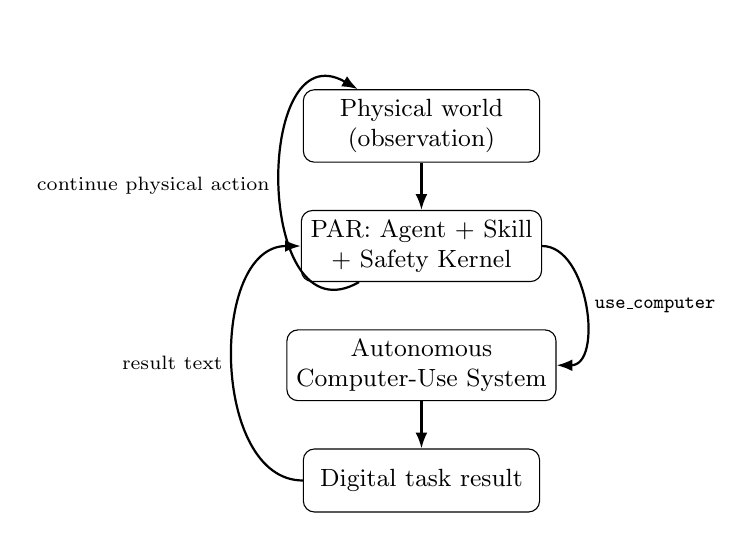
\begin{tikzpicture}[
  node distance=6mm,
  box/.style={draw, rounded corners, align=center, minimum height=8mm, minimum width=30mm, font=\small},
  arr/.style={-{Latex[length=2mm]}, thick}
]
\node[box] (world) {Physical world\\(observation)};
\node[box, below=of world] (par) {PAR: Agent + Skill\\+ Safety Kernel};
\node[box, below=of par] (acs) {Autonomous\\Computer-Use System};
\node[box, below=of acs] (result) {Digital task result};

\draw[arr] (world) -- (par);
\draw[arr] (par.east) to[out=0,in=0] node[right, font=\scriptsize] {\texttt{use\_computer}} (acs.east);
\draw[arr] (acs) -- (result);
\draw[arr] (result.west) to[out=180,in=180] node[left, font=\scriptsize] {result text} (par.west);
\draw[arr] (par) to[out=-150,in=150,looseness=1.6] node[left, font=\scriptsize] {continue physical action} (world);
\end{tikzpicture}
\caption{The Reach delegation cycle. PAR's planner proposes an action; a
\texttt{use\_computer} action is safety-checked, dispatched to the ACS, and
its result rejoins PAR's loop so the robot's physical task can continue.}
\label{fig:cycle}
\end{figure}

\subsection{Physical Agent Runtime (PAR)}
PAR implements a fixed loop -- \textit{Observation~$\rightarrow$~Agent~
$\rightarrow$~Skill~$\rightarrow$~Safety~$\rightarrow$~Action} -- around
three data types: an \texttt{Observation} (robot state and detected
objects), an \texttt{Action} (a named skill with parameters), and a
\texttt{Capability} (a skill's declared name, description, input schema,
risk level, and the environment profiles it is valid under). A
\texttt{Planner} maps a goal and the current observation to the next
\texttt{Action}; we use interchangeably a deterministic
keyword-matching planner for testing and an LLM tool-use planner
(Claude or Gemini, following the ReAct pattern~\cite{yao2023react}) for
open-ended goals, both implementing the same interface so the surrounding
runtime is agnostic to which one is in use.

\subsection{Safety Kernel}
Every proposed action passes a two-stage check before it executes. The
\textit{admission} stage rejects a capability outright if the runtime is
in an emergency-stopped state or the capability is not registered for the
active environment profile. The \textit{policy} stage evaluates the
specific action against that profile's constraints (workspace bounds,
collision margin against currently-detected objects, velocity limits) and
returns one of four outcomes: \textsc{Allow}, \textsc{Modify} (e.g.\ a move
target is speed-clamped to a reachable distance), \textsc{Deny}, or
\textsc{Escalate} to a human-approval callback. A denial is fed back to the
planner rather than aborting the task, so the agent re-plans around it --
Algorithm~\ref{alg:safety} summarizes the check for the capability at the
center of this paper.

\begin{algorithm}[t]
\caption{Safety check for a proposed action}
\label{alg:safety}
\begin{algorithmic}[1]
\REQUIRE action $a$, observation $o$, capability $c$, profile $p$
\IF{emergency stop engaged}
  \RETURN \textsc{Deny}
\ENDIF
\IF{$p$.name $\notin$ $c$.env\_profiles}
  \RETURN \textsc{Deny} \COMMENT{admission stage}
\ENDIF
\IF{$c$.risk $=$ \textsc{High} \AND $p$.approval\_required}
  \RETURN \textsc{Escalate}
\ENDIF
\IF{$a$.skill $=$ \texttt{move}}
  \RETURN CheckMove$(a, o, p)$ \COMMENT{workspace / collision / velocity}
\ENDIF
\RETURN \textsc{Allow}
\end{algorithmic}
\end{algorithm}

We mark \texttt{use\_computer} as \textsc{High} risk. Combined with a
profile that requires approval, this forces a human-approval escalation
before any delegation to the ACS in a real-robot deployment; under a
permissive simulation profile it runs unattended, which is what let us
validate the loop without a human in it for every step.

\subsection{Autonomous Computer-Use System (ACS)}
The ACS (CollectiveOS in our implementation) runs a perceive--plan--act--verify
loop over a real desktop: it captures a screenshot and the platform
accessibility tree, plans a short sequence of sub-steps with a
vision-language model, grounds and executes each step through UI
automation or browser control, and verifies the action changed the screen
as expected before continuing -- the same shape of loop used by GUI-agent
benchmarks and systems~\cite{zhou2023webarena,deng2023mind2web,hong2023cogagent,anthropic2024computeruse}.
Write-flavored actions (send, delete, purchase, \ldots) are meant to pause
for human-in-the-loop confirmation when the ACS is driven through its own
chat interface; critically, that confirmation gate is \emph{not} wired
into the robot-facing endpoint described next, which is why PAR's own
safety kernel is load-bearing for this integration rather than a
convenience.

\subsection{The Bridge}
PAR exposes computer use to its planner as a single capability,
\texttt{use\_computer}, taking one parameter (\texttt{task}, a natural-language
description of the digital step). When the planner selects it and the
safety kernel allows or approves it, a robot-interface wrapper forwards the
request over a WebSocket connection to the ACS's robot-facing endpoint,
which runs its computer-use loop synchronously and replies with a status
and a natural-language result (Table~\ref{tab:protocol}). The reply is
translated back into PAR's own \texttt{ActionResult} type, so from the rest
of PAR's perspective a delegated computer step looks exactly like any other
skill's result -- success or failure, with a message the planner can read
and react to. Every such run is also recorded by the ACS as an
imitation-learning demonstration (a before-screenshot paired with the
action taken at each step), which is the data trail this delegation
protocol produces toward a robot eventually \emph{learning} to use a
computer rather than only delegating it.

\begin{table}[t]
\centering
\caption{Wire protocol between PAR and the ACS (JSON over WebSocket)}
\label{tab:protocol}
\begin{tabular}{@{}p{0.46\linewidth}p{0.46\linewidth}@{}}
\toprule
\textbf{Robot $\rightarrow$ ACS} & \textbf{ACS $\rightarrow$ Robot} \\
\midrule
\texttt{\{"type":"task",} & \texttt{\{"type":"reply",} \\
\texttt{~"text":\textless task\textgreater\}} & \texttt{~"text":\textless result\textgreater,} \\
 & \texttt{~"status":\textless done\textbar error\textgreater\}} \\
\bottomrule
\end{tabular}
\end{table}

A network failure, a timeout, or an authentication error is caught at the
bridge and returned as a normal failed result rather than an exception,
so a delegation that cannot reach the ACS is something the planner can
observe and re-plan around, in keeping with the safety kernel's own
denial-is-recoverable design.

\subsection{Physical Simulation Integration}
To evaluate whether the safety kernel's physical checks (workspace bounds,
collision margin) behave sensibly against something more than an
in-memory mock, we bridged PAR to a physically-simulated differential-drive
robot in Webots~\cite{michel2004webots}. PAR already supports a ROS~2
robot interface with a pure, transport-agnostic JSON mapping between its
\texttt{Observation}/\texttt{Action} types and a wire payload; because our
development environment had no official ROS~2 build for its OS/CPU
combination and very little free disk for a full ROS~2 or virtual-machine
install, we reused that same JSON mapping over a plain WebSocket to an
external Webots controller process instead of ROS~2 topics. The bridge
controller runs a point-and-shoot controller for the \texttt{move}
capability -- rotate in place to face the target within a heading
tolerance, drive straight while re-checking heading, stop within a
distance tolerance -- and answers \texttt{detect}/\texttt{inspect} via
direct supervisor queries of known objects' world positions, which are the
same positions the safety kernel's collision check consumes, so a
collision denial exercises identically whether the robot behind PAR is the
in-memory mock or the simulated one.

\section{Implementation}
PAR (Pulse) and the ACS (CollectiveOS) are independent Python code bases
communicating only over the protocols described above; each also embeds
its own LLM client (Claude or Gemini for PAR's planner, Gemini for the
ACS's perception/planning) behind an interface so either can be swapped.
The ACS's own conversational surface is a FastAPI service with a
LangGraph-based task loop; PAR is a plain library with no server component
of its own -- it is a runtime a robot's control process links against
directly. Table~\ref{tab:stack} summarizes the stack.

\begin{table}[t]
\centering
\caption{Implementation stack}
\label{tab:stack}
\begin{tabular}{@{}ll@{}}
\toprule
\textbf{Concern} & \textbf{Choice} \\
\midrule
Language & Python \\
Data validation & Pydantic \\
PAR planners & Rule-based; Claude / Gemini tool-use \\
ACS API layer & FastAPI, WebSocket \\
ACS task loop & LangGraph \\
ACS screen control & Platform accessibility tree, browser automation,\\
 & pointer/keyboard automation \\
PAR $\leftrightarrow$ ACS transport & WebSocket, JSON payloads \\
Physical simulation & Webots \\
\bottomrule
\end{tabular}
\end{table}

\section{Preliminary Evaluation}
We report what has and has not been exercised so far; this is a systems
validation, not a benchmark result.

\textbf{Live delegation.} We ran a read-only task end to end: PAR's
runtime, under the safety kernel's escalation gate, delegated ``which
application is currently in the foreground?'' to a live instance of the
ACS. The ACS's vision-language model correctly identified the foreground
application, and the result returned through PAR's normal
\texttt{ActionResult} path. A transient upstream rate-limit error on a
first attempt surfaced as an ordinary failed result rather than a crash,
and a retry succeeded -- the behavior the bridge's error handling is
designed to produce.

\textbf{Unit and integration tests.} PAR's test suite (data models, the
safety kernel's four outcomes, the planner interface, the bridge's
dispatch logic against a fake ACS collaborator) passes in full. The ACS's
test suite, including regression tests we added for its robot-facing
WebSocket endpoint after finding and fixing an authentication bug that had
made that endpoint entirely unreachable, likewise passes in full.

\textbf{Simulated-robot bridge.} No physical Webots installation was
available in the development environment while the simulation bridge was
built. We instead validated its control logic against a hand-written fake
implementing real differential-drive kinematics: the point-and-shoot
\texttt{move} controller converges to arbitrary target waypoints from that
simulated kinematic model, and the WebSocket request/response path --
including the threading handoff between the network-facing thread and the
single thread that must own the simulator's own API -- was exercised end
to end against a real WebSocket server and client. The Webots-specific API
surface itself (exact device and node names, coordinate-system handling)
remains unverified against a real installation.

Table~\ref{tab:eval} summarizes.

\begin{table}[t]
\centering
\caption{What has been verified, and how}
\label{tab:eval}
\begin{tabular}{@{}p{0.32\linewidth}p{0.32\linewidth}p{0.24\linewidth}@{}}
\toprule
\textbf{Component} & \textbf{Method} & \textbf{Result} \\
\midrule
PAR core (skills, safety kernel) & Unit tests & Pass \\
ACS robot-facing endpoint & Unit + integration tests & Pass (after fix) \\
Bridge dispatch logic & Unit tests, fake ACS & Pass \\
Live delegation & Manual, real ACS instance & Correct answer \\
Simulated-robot control loop & Scripted test, kinematic fake & Converges \\
Simulated-robot on real Webots & --- & Not yet run \\
\bottomrule
\end{tabular}
\end{table}

\section{Discussion and Limitations}
The current ROS~2 robot interface executes fire-and-forget, with no
completion acknowledgement from the physical robot -- a limitation we
inherited rather than fixed, since our simulation work deliberately
avoided that interface. A real deployment migrating from the WebSocket
bridge to ROS~2 (on hardware where ROS~2 is available) should close that
gap rather than carry it forward. Delegation so far has only been driven
by a scripted or rule-based planner selecting \texttt{use\_computer}; we
have not yet evaluated whether an LLM planner reliably chooses to delegate
\emph{only} when a step genuinely needs a computer, which is the more
interesting and harder question this architecture is meant to eventually
answer. Evaluation is presently a single manual run rather than a
benchmark suite; adapting a GUI-agent benchmark such as
WebArena~\cite{zhou2023webarena} or Mind2Web~\cite{deng2023mind2web} to be
invoked through a robot planner, rather than directly, is natural future
work. Finally, the current authentication between PAR and the ACS is a
single shared secret, adequate for one robot and one ACS instance in
development but not for a multi-robot or multi-tenant deployment.

\section{Future Work}
Immediate priorities are: (1) completing a hardware-in-the-loop
verification pass once a physical Webots installation is available, fixing
whatever real-API mismatches surface; (2) measuring how reliably an LLM
planner chooses \texttt{use\_computer} only when appropriate, ideally
against a held-out set of mixed physical/digital tasks; (3) extending the
simulated robot from a wheeled platform to a manipulator so that
\texttt{pick}/\texttt{place} delegation can be validated with real
grasping rather than state-only bookkeeping; and (4) exploring imitation
learning directly over the demonstrations the ACS already records during
delegated runs, which is the step that would turn this from a robot that
\emph{delegates} computer use into one that is, in the imitation-learning
sense, \emph{learning} to use a computer.

\section{Conclusion}
Reach shows that a robot's need to occasionally use a computer does not
require folding computer-use competence into the robot's own policy. A
small, explicit capability, gated by a two-stage safety kernel with a
human-escalation path, is enough to compose a physical agent runtime with
an independently-built autonomous computer-use system, and the same
schema-preserving approach extends to a physically-simulated robot without
requiring a full ROS~2 toolchain. The reference implementation is open,
tested, and validated on one live task end to end; the honest next step is
broader, harder validation -- on real simulator hardware, against
benchmark tasks, and with the planner itself deciding when to reach for
the computer.

\section*{Acknowledgment}
This system and this paper were developed with the assistance of Claude
(Anthropic).

\bibliographystyle{IEEEtran}
\begin{thebibliography}{99}

\bibitem{ahn2022saycan}
M.~Ahn \textit{et al.}, ``Do As I Can, Not As I Say: Grounding Language in
Robotic Affordances,'' \textit{arXiv preprint arXiv:2204.01691}, 2022.

\bibitem{huang2022zeroshot}
W.~Huang, P.~Abbeel, D.~Pathak, and I.~Mordatch, ``Language Models as
Zero-Shot Planners: Extracting Actionable Knowledge for Embodied Agents,''
in \textit{Proc. ICML}, 2022, arXiv:2201.07207.

\bibitem{driess2023palme}
D.~Driess \textit{et al.}, ``PaLM-E: An Embodied Multimodal Language
Model,'' in \textit{Proc. ICML}, 2023, arXiv:2303.03378.

\bibitem{brohan2023rt2}
A.~Brohan \textit{et al.}, ``RT-2: Vision-Language-Action Models Transfer
Web Knowledge to Robotic Control,'' \textit{arXiv preprint
arXiv:2307.15818}, 2023.

\bibitem{yao2023react}
S.~Yao \textit{et al.}, ``ReAct: Synergizing Reasoning and Acting in
Language Models,'' in \textit{Proc. ICLR}, 2023, arXiv:2210.03629.

\bibitem{schick2023toolformer}
T.~Schick \textit{et al.}, ``Toolformer: Language Models Can Teach
Themselves to Use Tools,'' in \textit{Proc. NeurIPS}, 2023,
arXiv:2302.04761.

\bibitem{shinn2023reflexion}
N.~Shinn, F.~Cassano, A.~Gopinath, K.~Narasimhan, and S.~Yao, ``Reflexion:
Language Agents with Verbal Reinforcement Learning,'' in \textit{Proc.
NeurIPS}, 2023, arXiv:2303.11366.

\bibitem{zhou2023webarena}
S.~Zhou \textit{et al.}, ``WebArena: A Realistic Web Environment for
Building Autonomous Agents,'' in \textit{Proc. ICLR}, 2024,
arXiv:2307.13854.

\bibitem{deng2023mind2web}
X.~Deng \textit{et al.}, ``Mind2Web: Towards a Generalist Agent for the
Web,'' in \textit{Proc. NeurIPS}, 2023, arXiv:2306.06070.

\bibitem{hong2023cogagent}
W.~Hong \textit{et al.}, ``CogAgent: A Visual Language Model for GUI
Agents,'' in \textit{Proc. CVPR}, 2024, arXiv:2312.08914.

\bibitem{wu2023autogen}
Q.~Wu \textit{et al.}, ``AutoGen: Enabling Next-Gen LLM Applications via
Multi-Agent Conversation,'' \textit{arXiv preprint arXiv:2308.08155}, 2023.

\bibitem{wang2023voyager}
G.~Wang \textit{et al.}, ``Voyager: An Open-Ended Embodied Agent with
Large Language Models,'' \textit{arXiv preprint arXiv:2305.16291}, 2023.

\bibitem{michel2004webots}
O.~Michel, ``Cyberbotics Ltd. Webots\texttrademark: Professional Mobile
Robot Simulation,'' \textit{International Journal of Advanced Robotic
Systems}, vol.~1, no.~1, pp.~39--42, 2004.

\bibitem{quigley2009ros}
M.~Quigley \textit{et al.}, ``ROS: an open-source Robot Operating
System,'' in \textit{ICRA Workshop on Open Source Software}, 2009.

\bibitem{todorov2012mujoco}
E.~Todorov, T.~Erez, and Y.~Tassa, ``MuJoCo: A physics engine for
model-based control,'' in \textit{Proc. IEEE/RSJ IROS}, 2012, pp.~5026--5033.

\bibitem{makoviychuk2021isaacgym}
V.~Makoviychuk \textit{et al.}, ``Isaac Gym: High Performance GPU-Based
Physics Simulation For Robot Learning,'' \textit{arXiv preprint
arXiv:2108.10470}, 2021.

\bibitem{amodei2016concrete}
D.~Amodei, C.~Olah, J.~Steinhardt, P.~Christiano, J.~Schulman, and
D.~Man{\'e}, ``Concrete Problems in AI Safety,'' \textit{arXiv preprint
arXiv:1606.06565}, 2016.

\bibitem{bai2022constitutional}
Y.~Bai \textit{et al.}, ``Constitutional AI: Harmlessness from AI
Feedback,'' \textit{arXiv preprint arXiv:2212.08073}, 2022.

\bibitem{tobin2017domain}
J.~Tobin \textit{et al.}, ``Domain Randomization for Transferring Deep
Neural Networks from Simulation to the Real World,'' in \textit{Proc.
IEEE/RSJ IROS}, 2017, arXiv:1703.06907.

\bibitem{peng2018simtoreal}
X.~B. Peng, M.~Andrychowicz, W.~Zaremba, and P.~Abbeel, ``Sim-to-Real
Transfer of Robotic Control with Dynamics Randomization,'' in \textit{Proc.
IEEE ICRA}, 2018, arXiv:1710.06537.

\bibitem{anthropic2024computeruse}
Anthropic, ``Developing a computer use model,'' Anthropic Technical
Report, 2024. [Online]. Available: \url{https://www.anthropic.com/news/developing-computer-use}

\end{thebibliography}

\end{document}
